\documentclass[conference]{IEEEtran}
\usepackage{graphicx}
\usepackage{array}
\usepackage{bigstrut}
\usepackage{rotating}
\usepackage{multirow}
\usepackage{booktabs}

\hyphenation{op-tical net-works semi-conduc-tor}

\title{Feeding Dynamic Behavior into Optimization: Simulation-based Multi-objective Overtime Planning}

<<<<<<< HEAD
\author{\IEEEauthorblockN{M{\'a}rcio de O. Barros\IEEEauthorrefmark{1},
=======
\author{\IEEEauthorblockN{M\'arcio de O. Barros\IEEEauthorrefmark{1},
>>>>>>> bebbc47c358f93b9cd6e01015a466bf90b44bbfe
						  Luiz Antonio O. de Araujo Jr\IEEEauthorrefmark{2}
        \IEEEauthorblockA{Federal University of the State of Rio de Janeiro\\
Av. Pasteur 458, CEP 22.290-240
Rio de Janeiro, Brazil
\\ \{marcio.barros\IEEEauthorrefmark{1}, luiz.araujojr\IEEEauthorrefmark{2}\}@uniriotec.br}
}}

\begin{document}

\setlength{\floatsep}{2pt}
\setlength{\textfloatsep}{0pt}
\setlength{\intextsep}{2pt}
\setlength{\belowcaptionskip}{0pt}
\setlength{\abovecaptionskip}{0pt}

\maketitle
\begin{abstract}
IT professionals are particularly subjected to working overtime due to difficulties in estimation, requirement specification, and measuring progress during a software development life-cycle. However, excessive overtime has detrimental effects on developers and the software they produce. This contrast creates the need for overtime-planning strategies to support project managers in taking the most from as few overtime hours as possible. In this paper we introduce a formulation for the overtime-planning problem which extends the state-of-art by taking into consideration both the positive effects of overtime on productivity and its negative effects on product quality. We use heuristic optimization to explore close to optimal overtime allocations under this formulation. We present an empirical study that compared our approach with current industrial practices and a similar formulation without negative effects. Results show that suppressing the flip-side of the gains brought by overtime may lead to wrong decisions. For instance, excessive allocation of overtime in large projects may lead a manager to underestimate project cost and makespan by 5\% and 3\%, respectively, due to longer testing activities required to fix the exceeding errors introduced by overtime. Evidence also supports an overtime-management strategy used in the industry that concentrates overtime in the second half of a project schedule to compensate for early delays - about 60\% of the overtime allocations produced under this strategy are optimal.
\end{abstract}

\begin{keywords}
Overtime planning; management; simulation.
\end{keywords}

\IEEEpeerreviewmaketitle

\section{Introduction}

Software engineers are professionals particularly subjected to working overtime, frequently without previous planning and in stressful, fire-fighting situations \cite{Frangos:1997}\cite{Hyman:2003}\cite{Houdmont:2011}. Difficulties associated to measuring the progress of a software project, late and volatile requirements, compressed schedules, and the 
 to shrink the time-to-market of new features \cite{Halliday:2011} are among the factors that contribute to the need of working overtime.

Excessive overtime affects both the life of developers and the software they produce. On regard of the developers, Nishikitani et al. \cite{NISHIKITANI:2005} have observed that overtime work in the IT sector presents positive correlation with depression, anger, and hostility indexes. They also observed an increase in equilibrium- and motor-related problems on Japanese workers from the IT sector subjected to long shifts \cite{karita:2006}. Regarding the outcome of developers' work, DeMarco \cite{demarco:1982} and Akula and Cusick \cite{akula:2008} relate overtime work with higher error generation rates in software projects. DeMarco and Lister  \cite{demarco:1999} also relate excessive overtime with increased personal attrition, which may reduce knowledge exchange amongst developers  \cite{Andreas:2005} and hamper the ability of a company to hold domain expertise and properly deal with developer turnover \cite{amin:2011}.

Problems related to overtime are not exclusive to the IT sector. Caruso \cite{caruso:2006} identified negative impacts of long work hours on American workers (fatigue, lack of alertness, weight gain, and health degradation), their families (delayed marriage and childbearing), and their employers (absenteeism due to illness, increased errors, and rework). The author also reminds about the extra cost incurred in order to identify and correct errors committed due to exhaustion (loss in quantity and quality of the goods produced and services provided by workers subjected to excessive overtime). Donald et al. \cite{Donald:2005} also found negative correlation between stress and productivity. Finally, overtime problems do not seem related to a specific culture, affecting Americans \cite{caruso:2006}\cite{Dembe:2005}, Brazilians \cite{fischer:2000}, Japanese \cite{karita:2006}, \cite{Sasaki:2007}, and Chinese \cite{Houdmont:2011}, to cite a few.

Despite the recent growth in works on search-based approaches to software project management \cite{ferrucci:2014}, there is a single previous study that addresses techniques to handle overtime planning \cite{Ferrucci:2013}. The approach uses a multi-objective genetic algorithm to identify the activities providing the best leverage in terms of reducing project makespan and risk of schedule overrun for an amount of overtime work. However, the former paper does not take account of the negative impact of overtime and the consequent rise in errors produced by tired developers. Previous studies \cite{demarco:1982}, \cite{akula:2008} have presented empirical evidence that this is an important factor: the work required to fix the exceeding errors may subdue the gains in schedule brought by working overtime, as well as increase project cost more than expected by stakeholders. The results presented in this paper confirm that ignoring the loss in work quality may lead project managers to incorrect decisions. Furthermore, the present paper finds empirical support for a practice currently used by the industry for overtime allocation.

This paper extends the state-of-the-art by taking into account the documented impact of overtime on the quality of the services provided by developers working in extended hours. It introduces a new formulation for the overtime planning problem which combines search-based optimization with a scenario-based simulation that takes into account an increase in the number of errors injected into a software product by a team working overtime. We compared our results to current practices on regard of overtime management and provide insights to support project managers on deciding when to use overtime work. By doing this, we found scientific support for an overtime-management practice used in the industry, that is, evidence aligned with project management intuition. Our results show that, on average, 60\% of the allocations that might be built according to this strategy are optimal. We also compared our results with a similar model that ignores the dynamics of error generation caused by overtime,  showing that wrong decisions may be taken if the increase in error generation rates is not taken into account. For instance, excessive allocation of overtime in large projects may lead a manager to underestimate project cost and makespan, respectively, by 5\% and 3\% due to longer testing activities required to fix the exceeding errors introduced by overtime. The primary contributions of this paper are:

\begin{enumerate}
\item We introduce a new formulation for the multi-objective overtime-planning problem that considers an increase in error generation rates due to fatigue. Our approach takes into account trade-offs among the number of overtime hours worked in a project, makespan, and cost;

\item We present an empirical study based on 6 real-world projects with up to 635 function-points in size. Results show that concentrating overtime hours in the second part of project schedules (a practice used in the industry) is a good strategy that can be improved by optimization;

\item We present evidence that the negative impact on product quality caused by overtime must be taken into account while selecting the overtime allocation for a project. A strategy that may be optimal if such impact is disregarded may not be the best choice if it is considered.
\end{enumerate}

This paper is divided into 7 sections, starting with this introduction. Section II presents our formulation for the overtime-planning problem and the simulator used to capture software project dynamics. Section III presents the proposed solution for the overtime-planning problem. Section IV presents the design of the experimental study carried out to evaluate the proposed solution. Section V presents and discusses the results collected from this study. Section VI presents related work and Section VII shows conclusions and future research directions regarding overtime planning.

\section{Problem Formulation}
The innovation in our overtime-planning problem (OPP) formulation on respect of previous works relates to capturing the dynamics of error generation and propagation throughout the sequence of activities comprising a software project. This allows estimating the effects of an increase in error generation rates due to excessive overtime and fatigue. To this end, we devised a strategy to build a project schedule from a set of work packages and use continuous simulation to emulate the dynamics of error propagation as the schedule is executed.

<<<<<<< HEAD
We depart from a set of work packages to be analyzed, designed, coded, and tested. A project is represented as an acyclic directed graph $<$WP, WPDEP$>$ consisting of a node set WP=\{$wp_1, wp_2, ..., wp_n$\} of work packages and an edge set WPDEP=\{($wp_i, wp_j$): i$\not=$j, 1$\leq$i$\leq$n, 1$\leq$j$\leq$n\} of precedence dependencies amongst work packages. Each $wp_i$ is described by the amount of effort required to elicit its requirements, the amount of effort to design it, code it, and test it as if these tasks were performed by a mean developer in a regular work environment. A work package is also described by the number of errors its requirements analysis, design, and coding activities might generate in a similar context. On Section II.B we discuss how these parameters were filled for our instances. Each dependence in WPDEP represents a work package ($wp_i$) whose development can only start after the requirements for a second work package ($wp_j$) are known.

From these work packages, we develop a project schedule. Our schedule is a partial order of software development activities on which four types of activities are created for each work package: requirement analysis, design, coding, and testing. A testing activity is always preceded by a coding activity, which is preceded by a design activity, which comes after a requirement analysis activity. These dependencies represent the basic workflow of modeling the problem, designing the solution, implementing its source-code, and testing its features. The schedule also includes dependencies amongst work packages: the requirements analysis activity for work package $wp_i$ cannot start before the requirements analysis activity for $wp_j$ is concluded for all $(wp_i, wp_j)$ pairs in WPDEP. 

A schedule is an acyclic directed graph $<$AC, ACDEP$>$ consisting of a node set AC=\{$a_1, a_2, ..., a_n$\} of activities and an edge set ACDEP=\{($a_i, a_j$): i$\not=$j,1$\leq$i$\leq$m,1$\leq$j$\leq$m\} of finish-start (FS) dependencies amongst activities. A FS dependency A$\rightarrow$B indicates that work on activity B can only start when activity A is finished. Each activity is classified as either requirement analysis, design, coding, or testing. Analysis, design, and coding activities are described by the expected effort required to produce their results and the expected number of errors they might generate if performed by a mean developer in a regular environment. Testing activities are described by the average effort required to identify and correct an error, which is collected from information data in work packages.

=======
We depart from a set of work packages, each to be analyzed, designed, coded, and tested. A project is represented as an acyclic directed graph $<$WP, WPDEP$>$ consisting of a node set WP = \{wp$_{1}$, wp$_{2}$, ..., wp$_{n}$\} of work packages and an edge set WPDEP = \{(wp$_{i}$, wp$_{j}$): i$\not=$j,1$\leq$i$\leq$n,1$\leq$j$\leq$n\} of precedence dependencies amongst work packages. Each wp$_{i}$ is described by the amount of effort required to elicit its requirements, the amount of effort to design it, code it, and test it as if these tasks were performed by a mean developer in a regular work environment. A work package is also described by the number of errors its requirements analysis, design, and coding activities might generate in a similar context. On Section II.B we discuss how these parameters were filled for our instances. Each dependence in WPDEP represents a work package (wp$_{i}$) whose development can only start after the requirements for a second work package (wp$_{j}$) are known.

From these work packages, we develop a project schedule. Our schedule is a partial order of software development activities on which four types of activities are created for each work package: requirement analysis, design, coding, and testing. A testing activity is always preceded by a coding activity, which is preceded by a design activity, which comes after a requirement analysis activity. These dependencies represent the basic workflow of modeling the problem, designing the solution, implementing its source-code, and testing its features. The schedule also includes dependencies amongst work packages: the requirements analysis activity for work package wp$_{i}$ cannot start before the requirements analysis activity for wp$_{j}$ is concluded for all (wp$_{i}$, wp$_{j}$) pairs in WPDEP. 

A project schedule is represented as an acyclic directed graph $<$ACT, ACDEP$>$ consisting of a node set ACT = \{a$_{1}$, a$_{2}$, ..., an\} of activities and an edge set ACDEP = \{(a$_{i}$, a$_{j}$): i$\not=$j,1$\leq$i$\leq$m,1$\leq$j$\leq$m\} of finish-start (FS) dependencies amongst activities. A FS dependency A$\rightarrow$B indicates that work on activity B can only start when activity A is finished. Each activity a$_{i}$ is classified as either requirement analysis, design, coding, or testing. Analysis, design, and coding activities are described by the expected effort required to produce its results and the expected number of errors they might generate if performed by a mean developer in a regular environment. Testing activities are described by the average effort required to identify and correct an error, which is collected from information provided in work packages.
>>>>>>> bebbc47c358f93b9cd6e01015a466bf90b44bbfe
We consider three objectives for overtime planning: the number of overtime hours (NOH), project makespan (MKS), and overall project cost (CST). OPP is formulated as a three objective decision problem in which makespan, cost, and overtime hours are conflicting objectives to be minimized. A candidate solution for the OPP is a sequence of numbers that represents the amount of daily overtime hours to be spent on each activity comprising the schedule. Our formulation is based on a 40-hours work week, accepts multiples of 30 minutes for overtime work, and limits the maximum amount of daily work to 12-hours turns, according to Brazilian law. Thus, for any given activity we may assign zero overtime, 30 minutes of overtime, one hour, one hour and 30 minutes, and so on up to four hours of daily overtime. Our first objective, NOH, is calculated as the sum of the amount of overtime hours assigned for each activity in the schedule.

The $<$ACT, ACDEP$>$ graph is comprised of a set of paths $\Pi$ denoting the precedence-respecting sequences of activities that must be executed to complete the project. Makespan is given by the longest path in $\Pi$ (critical path) and is calculated by Equation (1). The duration of an activity is calculated by a simulator according to the characteristics of the activity and its execution setup (including the number of daily overtime hours assigned to it). The simulator calculates the number of errors produced by each development activity and propagates these errors to succeeding activities. For testing activities, the simulator calculates the effort required to identify and correct all errors received from former activities.

\setlength\abovedisplayshortskip{0pt}
\setlength\belowdisplayshortskip{0pt}
\begin{small}
\begin{equation}
MKS = MAX_{p\in\Pi} (\sum_{a_{i} \in p} Duration (a_{i}))
\end{equation}
\end{small}

The last objective, project cost (CST), is the sum of each activity's cost. The cost of an activity depends on the number of regular work hours and overtime hours its developers consume to produce its expected results and is related to the duration calculated by the simulator. Again, we modeled the problem according to Brazilian laws: if a regular working hour costs X, each of the first two overtime hours costs 120\%.X and the next two overtime hours cost 150\%.X each.


\subsection{Simulation Mechanism}
Simulation is the imitation of the behavior presented by a real-world process or system over time \cite{Banks:2000}. It supports predicting and understanding the behavior of complex systems, containing hundreds or thousands of interconnected components. Simulation is useful because the number of components and the complexity of the data and control exchange among them usually hampers our ability to interpret system behavior by intuition or analytical reasoning.

Simulation has been used to support understanding the behavior of large software systems. Continuous \cite{Forrester:1961} and discrete-event \cite{Ross:1990} simulation are the most used mechanisms to simulate software projects, though other mechanisms, such as state-based \cite{harel:1990} and rule-based \cite{Drappa:1999} simulation, have also been tested. Nonetheless, even the most frequently used simulation mechanisms have limitations, such as the inability to separate general from situation-specific behavior \cite{Barros:2002}, difficulties to separate the parts of a model related to a given component, to model simultaneous consumption of limited resources by two or more clients (continuous simulation), and to model state changes unrelated to an event (event-driven).
<<<<<<< HEAD

To overcome some of these problems, we have designed an object-oriented, continuous-time simulator to model the effects of overtime in software projects and predict project behavior (cost and makespan) accordingly. The simulator is based on three constructs: {\it simulation objects}, {\it resources}, and {\it scenarios}. Instead of creating a specific syntax to represent these elements, we relied on the Java programming language to describe and execute them. Designing the simulator in Java also simplified its integration to the heuristic search framework we have used in our experimental study.
=======

To overcome some of these problems, we have designed an object-oriented, continuous-time simulator to model the effects of overworking in software projects and predict project behavior (cost and makespan) accordingly. The simulator is based on three constructs: simulation objects, resources, and scenarios. Instead of creating a specific syntax to represent these elements, we relied on the Java programming language to describe and execute them. Designing the simulator in Java also simplified its integration to the heuristic search framework we have used in our experimental study.

Simulation objects are the elements whose behavior we want to simulate. They represent the nodes of a directed and acyclic graph whose edges denote precedence dependencies amongst simulation objects. They are initialized before the simulation starts and thereafter kept dormant until all their dependencies have been processed. Then, they become alive and start participating in the simulation until signaling their conclusion to the simulator. Simulation ends when all objects presented to the simulator are finished.

Time is managed in a continuous fashion. Simulation starts at time zero and is comprised of consecutive simulation steps, each advancing the simulator's clock by an infinitesimal increment. At each step, all alive simulation objects are allowed to update their internal state. The internal state of an object is defined according to the relevant characteristics of the real-world element it represents in the simulation. The behavior of an object is thus represented by the changes observed in its internal state during the simulation.

Simulation objects are Java objects that implement an interface defining a protocol through which they are controlled by the simulator. The internal state of an object is kept in its instance variables. Internal state adjustment operations are coded in methods activated by the simulator: \textit{init()}, to initialize the simulation object at time zero; \textit{start()}, called when all dependencies for an object are finished; \textit{step()}, called at each simulation step; and \textit{finish()}, called when the object signals its conclusion.

During a simulation step, simulation objects may use resources. A resource has a limited amount of materials or capabilities that can be consumed by simulation objects. These materials or capabilities are refilled before each simulation step. An object may request part of the resource's stock and adjust its internal state accordingly to its availability. The simulator controls the usage of limited resources by different simulation objects running in parallel. To model a software project, simulation objects represent an activity network with FS dependencies. The developers available to work on activities are resources whose amount of work is limited to a certain number of hours per day and is renewed in a daily basis. Developers are assigned to activities and if two or more activities executing in parallel share the same developer, only one of them will use the developer's capabilities at a time.

\textit{Scenarios} are used to represent complementary behavior that may be imposed to certain simulation objects. A scenario is written to influence a certain type of simulation object and only participates in the simulation if activated on one or more objects of that type. Scenarios can query and update the internal state of their associated objects before and after each event on which the objects update their internal state (\textit{start}, \textit{step}, \textit{finish}). Scenarios can be used to represent managerial decisions imposed to a subset of a software project's activities. They are reusable model components that modify the behavior of their related simulation object according to the policy they represent. For the purpose of the OPP, a scenario was developed to represent the effects of overtime while a base model describes the expected behavior for a project, its activities and developers as if uninfluenced by managerial policies and decisions (such as overtime allocation).
>>>>>>> bebbc47c358f93b9cd6e01015a466bf90b44bbfe

{\it Simulation objects} are the elements whose behavior we want to simulate. They represent the nodes of a directed and acyclic graph whose edges denote precedence dependencies amongst simulation objects. They are initialized before the simulation starts and thereafter kept dormant until all their dependencies have been processed. Then, they become alive and start participating in the simulation until signaling their conclusion to the simulator. Simulation ends when all objects presented to the simulator are finished.

Time is managed in a continuous fashion. Simulation starts at time zero and is comprised of consecutive {\it simulation steps}, each advancing the simulator's clock by an infinitesimal increment. At each step, all alive simulation objects are allowed to update their internal state. Simulation objects are Java objects that implement an interface defining a protocol through which they are controlled by the simulator. Their state is defined by the relevant characteristics of the real-world element they represent in the simulation. An object's state is kept in its instance variables. State adjustment operations are coded in methods activated by the simulator: {\it init()}, to initialize the object at time zero; {\it start()}, called when all dependencies for an object are finished; {\it step()}, called at each simulation step; and {\it finish()}, called when the object signals its conclusion. The behavior of an object is represented by the history of changes observed in its internal state during the simulation.

During a simulation step, objects may use resources. A {\it resource} has a limited amount of materials or capabilities that can be consumed by simulation objects. These materials or capabilities are refilled before each simulation step. An object may request part of the resource's stock and adjust its internal state accordingly to its availability. The simulator controls the usage of limited resources by different simulation objects running in parallel. To model a software project, simulation objects represent an activity network with FS dependencies. The developers available to work on activities are resources whose amount of work is limited to a certain number of hours per day and is renewed in a daily basis. Developers are assigned to activities and if two or more activities executing in parallel share the same developer, only one of them will use the developer's capabilities at a time.

Scenarios are used to represent complementary behavior that may be imposed to certain simulation objects. A scenario is written to influence a certain type of simulation object and only participates in the simulation if activated on one or more objects of that type. Scenarios can query and update the internal state of their associated objects before and after each event on which the objects update their internal state ({\it start}, {\it step}, {\it finish}). Scenarios can be used to represent managerial decisions imposed to a subset of a software project's activities. They are reusable model components that modify the behavior of their related simulation object according to the policy they represent. For the purpose of the OPP, a scenario was developed to represent the effects of overtime while a base model describes the expected behavior for a project, its activities and developers as if uninfluenced by managerial policies and decisions (such as overtime allocation).

\subsection{The Base Model}
The base simulation model is comprised of activities and developers. Activities are simulation objects linked to each other by precedence dependencies. An activity is available for simulation as soon as its precedent activities are concluded. Developers are resources who can spend a limited amount of work on each simulation step. They are characterized by their productivity and error generation rates.

Activities are separated into development and testing activities. Development activities are described by an expected amount of work to be performed (in developer-hours) and an amount of errors expected to be generated while this work is performed. The duration of a given activity depends on the amount of work to be performed and the productivity of the developer assigned to it. We calibrated the model using data from Jones \cite{Jones:2000}. Given a work package measured in function-points (FP), Jones \cite{Jones:2000} presents average distributions of effort required for each development phase. For instance, for projects of about 1,000 function-points, requirement analysis activities consume 7\% of project effort, design activities consume about 10\%, coding activities consume about 30\%, and testing consumes 30\%. The remaining effort is related to management, documentation, and other activities. In our model, this effort is proportionally distributed among the analysis, design, coding, and testing activities. Given this distribution, the size of a work package, and an average productivity of 27.8 function-points per developer-month \cite{Jones:2000}, we calculate the expected duration for each activity.

Error dynamics is trickier. When an activity starts, it collects all errors produced by its former activities (if any) carrying them toward the end product. Abdel-Hamid and Madnick \cite{Abdel-Hamid:1991} present a model for error reproduction which states that errors inherited by an activity are not only forwarded to succeeding activities, but they contribute to the generation of new errors. Jones \cite{Jones:2000} suggests that the average number of defects introduced by each kind of activity is 1 error/FP in requirement analysis, 1.25 errors/FP in design, and 1.75 errors/FP in coding activities. Based on these data, our model assumes that each activity introduces 1 new error/FP, design activities regenerate 25\% of errors it receives from analysis, and coding regenerates 33\% of the errors received from design. These regeneration rates lead to the mark of 4.0 errors/FP on average after the implementation and are compatible with the former model \cite{Abdel-Hamid:1991} and source \cite{Jones:2000}.

Testing activities receive the results of development activities and aim at identifying and correcting the errors introduced in the product. These activities are characterized by the average effort required to identify and correct an error. Their duration depends on this parameter along with the assigned developer’s productivity. Given the amount of work expected to be invested in the testing phase \cite{Jones:2000} (i.e., 30\% of total effort for 1,000 FP projects) and the expected number of errors reaching this activity in a regular situation (4 errors/FP), we calculate the average time required to identify and correct each error and use this value on testing activities.

\subsection{A Scenario for Overtime}

<<<<<<< HEAD
The scenario used in our simulation describes the dynamics of working overtime and its influence on developer's productivity and error generation rates. If a developer is expected to work more than 8 hours per day in a given activity, his productivity will be increased proportionally to the extra number of work hours, reaching up to a 50\% increase if working to the upper limit of 12 hours per day. However, according to deMarco's law \cite{demarco:1999}, a developer working more than the regular daily hours may produce software below the quality standard. The more hours a developer works, the more tired he becomes. Tired developers become less careful to the work they are performing and, consequently, they tend to introduce more errors in the software. We have used data from \cite{Abdel-Hamid:1991}  to estimate the increase in the number of errors produced according to the number of hours worked by a developer. Such data suggest that software quality tends to deteriorate if developers work more than 9 hours/day and that a developer working 12 hours/day commits 50\% more errors than while working on a regular shift.
=======
The scenario used in our simulation describes the dynamics of working overtime and its influence on developer's productivity and error generation rates. If a developer is expected to work more than 8 hours per day in a given activity, his productivity will be increased proportionally to the extra number of work hours, reaching up to a 50\% increase if working to the upper limit of 12 hours per day. However, according to de Marco’s law \cite{demarco:1999}, a developer working more than the regular daily hours may produce software below the quality standard. The more hours a developer works, the more tired he becomes. Tired developers become less careful to the work they are performing and, consequently, they tend to introduce more errors in the software. We have used data from \cite{Abdel-Hamid:1991}  to estimate the increase in the number of errors produced according to the number of hours worked by a developer. Such data suggest that software quality tends to deteriorate if developers work more than 9 hours/day and that a developer working 12 hours/day commits 50\% more errors than while working on a regular shift.
>>>>>>> bebbc47c358f93b9cd6e01015a466bf90b44bbfe

\section{Solution Approach}
Our solution uses the NSGAII algorithm for optimization along with the simulator described in Section II. NSGAII \cite{deb:2002} is a multi-objective genetic algorithm based on a ranking procedure which classifies candidate solutions according to their dominance. A candidate solution is described by the values calculated for the objectives of interest under that solution. In our case, these objectives are the number of overtime hours, project makespan, and project cost, all to be minimized. A solution A is said to dominate a solution B if the values of all objectives in A are no greater than the respective objectives in B and at least one objective is smaller in A than in B. Non-dominated solutions are assigned a rank of 1; solutions dominated only by non-dominated solutions are assigned a rank of 2; solutions dominated only by the former are assigned a rank of 3, and so on. The algorithm evolves a population over a number of generations, applying crossover, mutation, and selection upon candidate solutions. The selection process prioritizes low-ranking solutions and, when a subset of solutions having the same rank must be selected, a density measure allows selecting candidate solutions covering the search space as uniformly as possible. 

As any heuristic algorithm, NSGAII has components that must be specified for a given problem. Three components are discussed below, while population size and stop criteria were subject of analysis and are discussed in the next section.

\noindent
\textbf{Representation}. A candidate solution for OPP is a sequence of m integer numbers, m being the number of activities. Each number in the solution pertains to the [0..8] integer interval and represents a multiple of 30-minutes overtime for a given activity. Thus, if the number 4 is assigned to activity A, A will receive 1.5 hours of overtime work. Each individual solution being evolved by NSGAII is evaluated through simulation. The simulator activates the overtime scenario upon each activity in the schedule according to the number of overtime hours assigned to that activity in the solution. Then, the simulator calculates the number of overtime hours, project makespan, and project cost for that solution.

\noindent
\textbf{Crossover}. We reused the crossover operator proposed by Ferrucci et al. \cite{Ferrucci:2013}. This operator was adopted because it was shown to outperform the one-point crossover operator commonly used in NSGAII for their formulation for the overtime planning problem. Instead of exchanging genetic material of two parents P$_{1}$ and P$_{2}$ after a point of cut C $\in$ [1..m], the resulting offspring O$_{1}$ and O$_{2}$ produced by this operator are defined by the equations below (given a random variable p with uniform distribution). The operator is executed with 50\% probability; otherwise, the parents are copied to the next generation. Parents are selected by binary tournament.

\setlength\abovedisplayskip{0pt}
\setlength\belowdisplayshortskip{0pt}
\begin{small}
\begin{equation}
O_{1}(g)=
\left \{
\begin{array}{ll}
P_{1}(g) & 1\leq g < C \\
max(P_{1}(g), P_{2}(g)) & C\leq g\leq m,p < 0.5 \\
min(P_{1}(g), P_{2}(g)) & C\leq g\leq m,p \geq 0.5 \\
\end{array}
\right.
\end{equation}

\setlength\abovedisplayshortskip{0pt}
\setlength\belowdisplayshortskip{0pt}
\small
\begin{equation}
O_{2}(g)=
\left \{
\begin{array}{ll}
P_{2}(g)& 1\leq g < C \\
P_{1}(g)+P_{2}(g) & C\leq g\leq m\\
\end{array}
\right.
\end{equation}
\end{small}

\noindent
\textbf{Mutation}. As in Ferrucci et al. \cite{Ferrucci:2013}, mutations are executed for all crossover offspring. Each gene of an offspring O is changed with 30\% probability, being assigned a new value in the [0..8] integer interval.

\section{Experimental Design}
This section explains the design of our empirical study, presenting research questions, the instances selected to address these questions, and the measurements used to compare solutions found under different configurations and algorithms.
\subsection{Research Questions}

In this section we present the research questions addressed by our study. They were designed to provide evidence on the validity, competitiveness, and usefulness of our approach.

\noindent
\textbf{RQ1 (Validation):} How does NSGAII perform if compared to random search on finding solutions for OPP? This is a "sanity check" to determine if our formulation allows a systematic search to outperform random search. If such cannot be verified, either the formulation is poorly designed, parameters are not adequate, or the problem is simple enough to allow a non-systematic procedure to find good solution.

\noindent
\textbf{RQ2 (Competitiveness):} How does NSGAII perform if compared to currently used overtime planning approaches? Besides beating random search, the proposed approach has to outperform current management practices related to overtime planning. In this sense, we compare the results produced by NSGAII with overtime planning practices used in the industry.

\noindent
\textbf{RQ3 (Usefulness):} Do results of overtime planning change if we consider the dynamics of error generation and the loss of quality caused by overtime? To address this issue, we compare the results produced by NSGAII with and without considering an increase in error generation due to overtime. Different results denote that a manager may pick a distinct overtime planning strategy if error dynamics are not considered.

\subsection{Software Projects Used in the Study}

Table I presents information about the selected instances for the experimental analysis. The {\it Transaction Functions} and {\it Data Functions} columns count, respectively, the number of transaction and data functions for each instance. These values are related to the number of function points of the instance, presented in the last column. The {\it Work Packages} column presents the number of groups on which the data and transaction functions distributed to form the project schedule.

% Table generated by Excel2LaTeX from sheet 'tabela 1'
\begin{table}[htbp]
  \centering
  \caption{Instances used in the experimental studies}
    \begin{tabular}
		{
			p{0.7cm} 
			>{\centering\arraybackslash}p{1.5cm} 
			>{\centering\arraybackslash}p{1.3cm} 
			>{\centering\arraybackslash}p{1.3cm} 
			>{\centering\arraybackslash}p{1.3cm}
		}
    \toprule
		Name & Transaction Functions & Data Functions & Work Packages & Function Points \\
    \midrule
    ACAD  & 39    & 7     & 10    & 185 \\
    WMET  & 48    & 7     & 11    & 225 \\
    WAMS  & 67    & 8     & 15    & 381 \\
    PSOA  & 65    & 9     & 18    & 290 \\
    OMET  & 129   & 22    & 21    & 635 \\
    PARM  & 98    & 21    & 27    & 451 \\
    \bottomrule
    \end{tabular}%
\end{table}%

ACAD is an academic administrative system that allows managing classes, students, registrations, and teachers in an university setting. WMET allows users to add meteorological observations to a database and provides weather-related reports. WAMS is a message routing system responsible for receiving and routing air traffic control messages. PSOA is a personnel management project used by a large company for authentication, authorization, and centralization of references from enterprise systems. OMET is a system which manages, stores, and delivers meteorological information, including messages and statistical information regarding the weather. PARM stores configuration and setting values used by other systems, allowing for fast configuration of user profiles and sharing configurations amongst distinct applications. 

ACAD was developed to support post-graduate programs in a Brazilian university and has been in use for more than 10 years. WMET, WAMS, and OMET were developed and are currently used to support air traffic control in Brazil. PARM and PSOA are used by the IT company in charge for government-managed retirement funds in Brazil.	

\subsection{Multi-Object Evaluation Measurements}
A comparison between two or more mono-objective heuristic search algorithms can rely on the values found by these algorithms for the fitness function guiding the optimization. However, a similar comparison for multi-objective algorithms cannot rely directly on objective values because each algorithm provides a curve of non-dominated solutions (a Pareto front) as its results. Therefore, comparing different algorithms implies comparing different Pareto fronts. 

To compare two Pareto fronts F$_{A}$ and F$_{B}$ we need surrogate measures of their quality. These measures are called {\it quality indicators}. A quality indicator receives a set of points defined in the objective space and produces a real number. The result for a given front F$_{A}$ can be compared to the result for a second front F$_{B}$, leading to conclusions about the quality of these fronts and, consequently, the algorithms and configurations that produced them. Quality indicators usually compare each front with a 'reference front' F$_{R}$ built from the non-dominated solutions of all Pareto fronts under comparison. The ideal reference front would be the optimal set of non-dominated solutions for a given instance, but these are rarely available for practical purposes. Thus, the union of all available fronts followed by the elimination of duplicate and dominated solutions is used as a proxy to the ideal reference front. 

Given F$_{R}$ and two fronts to be compared a number of quality indicators can be defined. They usually address two properties of Pareto fronts: convergence and diversity. Convergence indicators measure how close a given front F$_{A}$ is to the reference front. Diversity indicators measure the amount of the solution space that is covered by a given front F$_{A}$. For the purpose of our study, we selected three indicators: Contributions (I$_{C}$), Hypervolume (I$_{HV}$), and Generational Distance $(I_{GD})$. These indicators are measured in the [0, 1] interval. I$_{C}$ is a convergence indicator that represents the proportion of solutions in a given front F$_{A}$ that also pertain to the reference front. Good Pareto fronts have high I$_{C}$, thus contributing heavily to the composition of F$_{R}$. I$_{HV}$ calculates the volume of the objective space that is covered by solutions of a given Pareto front \cite{Durillo:2009}. It mixes convergence to the reference front and diversity amongst the selected solutions comprising a given front. High-quality Pareto fronts present high hypervolume, thus covering a large extension of the objective space. Finally,  is a convergence indicator that measures the distance between a front and the reference front \cite{vanveldhuizen:1998}. Good fronts are closer to the reference front and thus present low generational distance.

\subsection{Parameter Setting for the Algorithm}
Section III presented the selected configuration for most components of NSGAII in order to fine-tune the algorithm to the OPP. However, two components were not addressed in that section because they required experimental analysis to be defined: the stop criteria, expressed in terms of a maximum number of fitness function evaluations NSGAII is allowed to perform while searching for solutions, and population size, that is, the size of the genetic pool evolved by NSGAII as a multiplier to the number of activities in a given instance.

To determine the most adequate stop criteria, we executed NSGAII for all selected instances with a maximum of 5,000, 10,000, 20,000, and 50,000 fitness evaluations. To properly account for the randomness inherent to heuristic search algorithms, the optimization was executed 50 times for each configuration and instance. Fifty thousand fitness evaluations was considered as an upper limit due to the time required to process each optimization cycle, particularly due to the cost of running the simulation on every fitness function evaluation. Afterwards, we built a reference front for each instance based on non-dominated solutions collected from all 50 cycles of all configurations under which the instance was optimized. Then, we calculated $I_{GD}$ for the front resulting from each optimization cycle based on the reference front. This led to a data frame containing 50 observations of $I_{GD}$ for each instance and configuration. Being bound to the [0..1] interval, quality indicators data cannot be normally-distributed and thus cannot be subjected to parametric statistical inference test. Thus, hereafter we will only use non-parametric tests. A Kruskal-Wallis non-parametric inference test was executed upon this data and found significant differences between configurations at 95\% significance level. A post-hoc analysis based on pair-wise comparisons through a Wilcoxon test using Bonferroni correction followed to find that there were significant differences among all configurations and the configuration using 50,000 fitness evaluations as stop criteria yielded smaller I$_{GD}$ for all instances. Thus, we used 50,000 fitness evaluations as stop criteria for all following analysis.

A similar procedure was used to determine the most adequate population size for each instance. First, we executed NSGAII for all instances with population sizes of $2m$, $4m$, and $8m$, $m$ being the number of activities for the instance and using 50,000 fitness evaluations as stop criteria. The optimization was executed 50 times for each configuration and instance, a reference front was built for each instance from the results of all 50 cycles, and we calculated $I_{GD}$ for the front resulting from each cycle, ending up with a data frame comprising 50 observations of $I_{GD}$ for each instance and configuration. A Kruskal-Wallis test was executed upon this data on an instance basis and found significant difference between configurations at 95\% level. The post-hoc analysis revealed significantly different results for all configurations on all instances and the configuration using $2m$ as population size yielded the best average for all instances. Therefore, we selected $2m$ as population size for all following analysis.

\section{Analysis and Discussion}
<<<<<<< HEAD
Below we present results obtained from our experiments to support answering the proposed research questions.
=======
Below we present results obtained from our experiments to support answering the proposed research questions. \linebreak
\textbf{RQ1:} To compare NSGAII to random search (RS), we ran 50 independent optimization cycles for both algorithms using the same stop criteria. NSGAII achieved higher I$_{HV}$, higher I$_{C}$, and lower  on all six instances compared to RS. Wilcoxon-Mann-Whitney tests applied on an instance basis found significant differences between results produced by the algorithms at 95\% significance level for all quality indicators and all instances. Standardized effect-sizes (non-parametric Vargha-Delaney \^A12 test) also indicate that NSGAII produces higher I$_{HV}$ and lower  in 100\% of the runs, while producing higher I$_{C}$ for more than 88\% of these runs. Thus, there is strong evidence that NSGAII outperforms RS while searching for solutions for the OPP and that our formulation and parameterization passes the "sanity check" implied in the first research question.\linebreak
\textbf{RQ2:} To address this question we compared our formulation for the OPP with three overtime management strategies (OMS) presented by Ferrucci et al. \cite{Ferrucci:2013} as reference practices from the industry: (i) "margarine" management (MAR) suggests spreading overtime hours evenly over all activities comprising the project schedule; (ii) Critical Path (CPM) suggests loading overtime onto the schedule's critical path to reduce completion time and risk of schedule overrun; and (iii) Second Half (SH) suggests loading overtime hours onto the later part of the project's schedule to compensate for delays introduced in early activities. 
>>>>>>> bebbc47c358f93b9cd6e01015a466bf90b44bbfe

\noindent
\textbf{RQ1:} To compare NSGAII to random search (RS), we ran 50 independent optimization cycles for both algorithms using the same stop criteria. NSGAII achieved higher I$_{HV}$, higher I$_{C}$, and lower I$_{GD}$ on all instances compared to RS. Wilcoxon-Mann-Whitney tests applied on an instance basis found significant differences between results produced by the algorithms at 95\% significance level for all quality indicators and all instances. Standardized effect-sizes (non-parametric Vargha-Delaney {\^A}12 test) also indicate that NSGAII produces higher I$_{HV}$ and lower I$_{GD}$ in 100\% of the runs, while producing higher I$_{C}$ for more than 88\% of these runs. Thus, there is strong evidence that NSGAII outperforms RS while searching for solutions for the OPP and that our formulation and parametrization pass the "sanity check" implied in RQ1.

\noindent
\textbf{RQ2:} To address this question we compared our formulation for the OPP with three overtime management strategies (OMS) presented by Ferrucci et al. \cite{Ferrucci:2013} as reference practices from the industry: (i) ''margarine'' management (MAR) suggests spreading overtime hours evenly over all activities comprising the schedule; (ii) Critical Path (CPM) suggests loading overtime onto the schedule's critical path to reduce completion time and risk of schedule overrun; and (iii) Second Half (SH) suggests loading overtime onto the later part of the schedule to compensate for delays introduced in early activities. 

The objectives of interest (NOH, MKS, and CST) were calculated for each OMS. Nine configurations were created for CPM, each loading a certain amount of daily overtime, from zero to four hours in 30-minute intervals, onto the critical path. The objectives were calculated for each configuration and a Pareto front was built from non-dominated solutions. A similar approach was taken for MAR and SH. The front produced for each OMS was compared with fronts produced by NSGAII over 50 independent optimization cycles on the basis of the quality indicators presented in Section IV.C.

A summary of values collected for each quality indicator and instance is presented in Table II. The distributions of these values are shown in the box-plots presented in Figure I. Data for NSGAII is shown in the form of mean $\pm$ standard deviation over the 50 cycles. Data for OMS is shown as a single value, since each OMS produced a single Pareto front for each instance. I$_{HV}$ and I$_{GD}$ for CPM on instances PARM and PSOA are not calculated because the OMS produced a Pareto front comprised of a single vertex, leading to undefined I$_{GD}$ and I$_{HV}$. Bold face OMS values were found significantly different from NSGAII using Bonferroni-adjusted Wilcoxon-Mann-Whitney inference tests at 95\% significance level. Bold face NSGAII values were found significantly different from all OMS using the same inference test. 

On regard on I$_{C}$, SH contributed with more vertices to the reference Pareto front than the average front produced by each cycle of NSGAII in 4 out of 6 instances. For the remaining instances, results slightly favor NSGAII, but without statistical significance in comparison with SH. On average, SH contributed with 5.2 solutions to the reference front, while NSGA-II contributed with 2.4 solutions. Each remaining OMS contributed with a single solution to the front (zero overtime). On regard of I$_{HV}$, NSGAII produced the best results except for the largest instance (PARM), on which it was significantly outperformed by SH. Finally, on regard of I$_{GD}$ NSGAII outperformed all OMS in 4 out of 6 instances, losing to SH on the OMET and PARM instances (the largest instances). For the latter, all solutions produced by SH were part of the reference front. Thus, we ratify the results presented by Ferrucci et al. \cite{Ferrucci:2013} in the sense that the CPM and margarine OMS are not competitive with optimization results. On the other hand, SH seems competitive and outperforms NSGAII in terms of closeness to the reference front on large instances.

\begin{figure*}
\centering
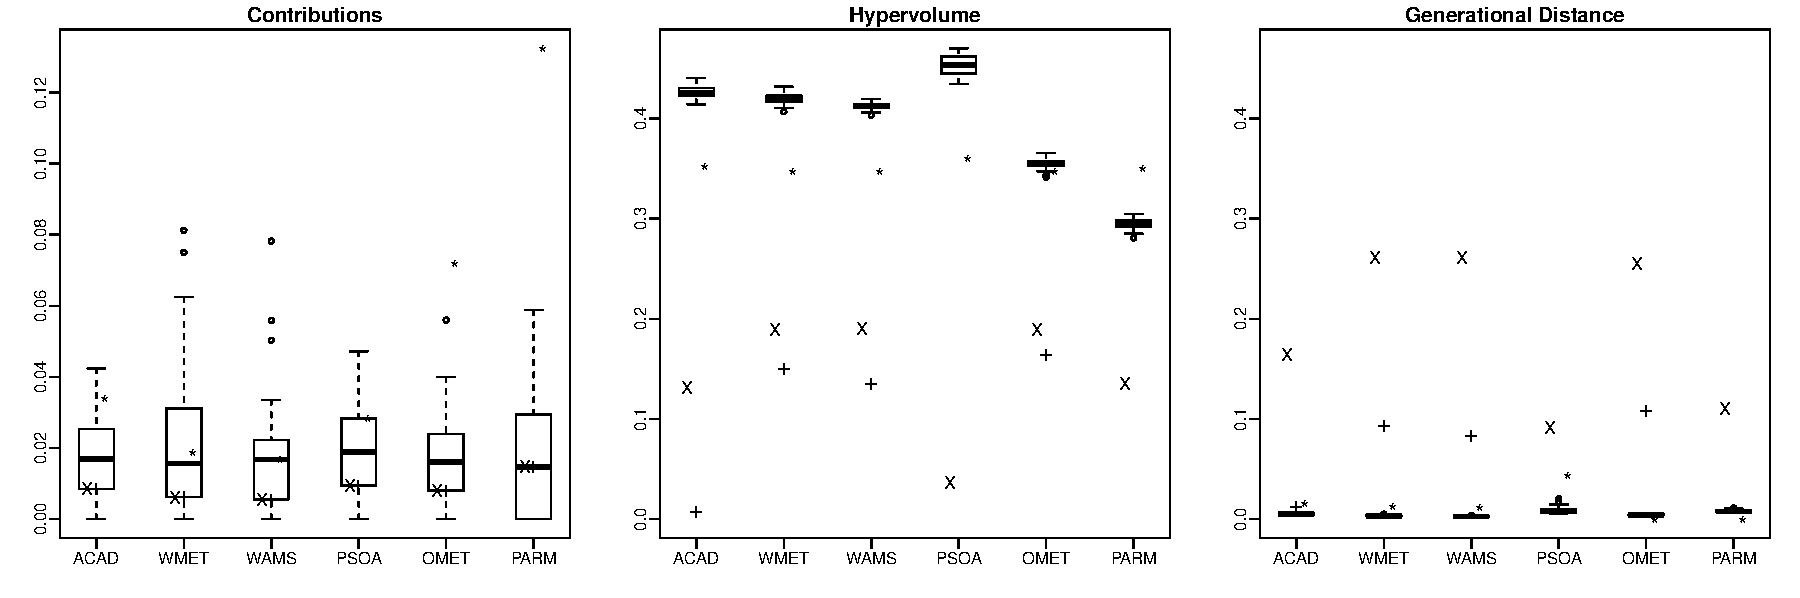
\includegraphics[width=18cm, height=5cm]{boxplots.pdf}
\caption{Boxplots for I$_{C}$ (left), I$_{HV}$ (middle) and I$_{GD}$ (right) quality indicators for NSGAII (boxplot), MAR ($\times$), SH ($\ast$), and CPM (+). The few solutions found under the second-half OMS are closer to optimal, though NSGAII produces a more diverse set of solutions.}
\end{figure*}

% Table generated by Excel2LaTeX from sheet 'tabela 2'
\begin{table}[htbp]
	\scriptsize
  \centering
  \caption{Quality indicator values for each instance under our approach (NSGAII) and the OMS. Pareto fronts produced under NSGAII present more diversity than those produced under the OMS. Solutions produced under the Second-Half OMS are closer to optimal for the largest instances.}
    \begin{tabular}{p{0.7cm} p{0.7cm} ccc}
    \toprule
    \textbf{Instance} & \textbf{Config} & \textbf{I$_{C}$} & \textbf{I$_{HV}$} & \textbf{I$_{GD}$} \\
    \midrule
    \multirow{4}[2]{*}{ACAD} & NSGAII & 0.0193 $\pm$ 0.0211 & \textbf{0.4262 $\pm$ 0.0063} & \textbf{0.0052 $\pm$ 0.0013} \\
          & MAR   & 0.0085 & 0.1318 & 0.1649 \\
          & SH    & \textbf{0.0339} & 0.3514 & 0.0153 \\
          & CPM   & 0.0085 & 0.0071 & 0.0127 \\\hline
    \multirow{4}[2]{*}{WMET} & NSGAII & 0.0196 $\pm$ 0.0186 & \textbf{0.4196 $\pm$ 0.0051} & \textbf{0.0034 $\pm$ 0.0005} \\
          & MAR   & 0.0062 & 0.1892 & 0.2612 \\
          & SH    & 0.0188 & 0.3464 & 0.0125 \\
          & CPM   & 0.0062 & 0.1502 & 0.0930 \\\hline
    \multirow{4}[2]{*}{WAMS} & NSGAII & 0.0197 $\pm$ 0.0158 & \textbf{0.4123 $\pm$ 0.0032} & \textbf{0.0028 $\pm$ 0.0003} \\
          & MAR   & 0.0056 & 0.1900 & 0.2613 \\
          & SH    & 0.0168 & 0.3470 & 0.0118 \\
          & CPM   & 0.0056 & 0.1357 & 0.0831 \\\hline
    \multirow{4}[2]{*}{PSOA} & NSGAII & 0.0194 $\pm$ 0.0141 & \textbf{0.4534 $\pm$ 0.0094} & \textbf{0.0091 $\pm$ 0.0032} \\
          & MAR   & 0.0094 & 0.0368 & 0.0918 \\
          & SH    & \textbf{0.0283} & 0.3600 & 0.0439 \\
          & CPM   & 0.0094 & n/a   & n/a \\\hline
    \multirow{4}[2]{*}{OMET} & NSGAII & 0.0186 $\pm$ 0.0125 & \textbf{0.3550 $\pm$ 0.0047} & 0.0042 $\pm$ 0.0003 \\
          & MAR   & 0.0080 & 0.1897 & 0.2557 \\
          & SH    & \textbf{0.0720} & 0.3469 & \textbf{0.0000} \\
          & CPM   & 0.0080 & 0.1637 & 0.1079 \\\hline
    \multirow{4}[2]{*}{PARM} & NSGAII & 0.0173 $\pm$ 0.0162 & 0.2949 $\pm$ 0.0054 & 0.0080 $\pm$ 0.0011 \\
          & MAR   & 0.0147 & 0.1358 & 0.1108 \\
          & SH    & \textbf{0.1324} & \textbf{0.3503} & \textbf{0.0000} \\
          & CPM   & 0.0147 & n/a   & n/a \\
    \bottomrule
    \end{tabular}%
\end{table}%

% Table generated by Excel2LaTeX from sheet 'tabela 3'
\begin{table}[htbp]
  \scriptsize
	\centering
  \caption{Effect-size for comparisons between NSGA and each OMS in terms of each quality indicator.}
    \begin{tabular}{p{0.6cm} p{0.6cm} p{0.65cm} p{0.65cm}p{0.65cm}p{0.65cm}p{0.65cm}p{0.65cm}}
    \toprule
    \textbf{QI} & \textbf{OMS} & \textbf{ACAD} & \textbf{WMET} & \textbf{WAMS} & \textbf{PSOA} & \textbf{OMET} & \textbf{PARM} \\
    \midrule
    \multirow{3}[1]{*}{I$_{C}$} & MAR   & 67\%  & 75\%  & 83\%  & 71\%  & 78\%  & 50\% \\
          & SH    & 17\%  & 41\%  & 53\%  & 29\%  & 0\%   & 0\% \\
          & CPM   & 67\%  & 75\%  & 83\%  & 71\%  & 78\%  & 50\% \\\hline
    \multirow{3}[2]{*}{I$_{HV}$} & MAR   & 100\% & 100\% & 100\% & 100\% & 100\% & 100\% \\
          & SH    & 100\% & 100\% & 100\% & 100\% & 96\%  & 0\% \\
          & CPM   & 100\% & 100\% & 100\% & n/a   & 100\% & n/a \\\hline
    \multirow{3}[2]{*}{I$_{GD}$} & MAR   & 100\% & 100\% & 100\% & 100\% & 100\% & 100\% \\
          & SH    & 100\% & 100\% & 100\% & 100\% & 0\%   & 0\% \\
          & CPM   & 100\% & 100\% & 100\% & n/a   & 100\% & n/a \\
    \bottomrule
    \end{tabular}%
\end{table}%

<<<<<<< HEAD
The {\^A12} effect-size was calculated for pair-wise comparisons between NSGAII and each OMS for all quality indicators. Results are presented in Table III, denoting the chances of NSGAII to produce higher I$_C$ and I$_{HV}$ and lower I$_{GD}$ than the related OMS. {\^A}12 is very high and favors NSGAII in almost all instances for I$_{HV}$ and I$_{GD}$ (except PARM for I$_{HV}$, OMET and PARM for I$_{GD}$). It strongly favors NSGAII in terms of $I_C$ if compared to MAR and CPM, except on PARM (a draw on effect-size among both OMS and NSGAII). On the other hand, {\^A}12 tells a different story for I$_{C}$ between NSGAII and SH, clearly favoring SH for almost all instances. 
=======
The \^A12 standardized effect-size was calculated for pair-wise comparisons between NSGAII and each OMS for all quality indicators. Results are presented in Table III, denoting the chances of NSGAII to produce higher IC and I$_{HV}$ and lower  than the related OMS. \^A12 is very high and favors NSGAII in almost all instances for I$_{HV}$ and  (except PARM for I$_{HV}$, OMET and PARM for I$_{GD}$). It strongly favors NSGAII in terms of IC if compared to MAR and CPM, except on instance PARM (a draw on effect-size among both OMS and NSGAII). On the other hand, \^A12 tells a different story for I$_{C}$ between NSGAII and SH, clearly favoring SH for almost all instances. 
>>>>>>> bebbc47c358f93b9cd6e01015a466bf90b44bbfe

Effect-sizes are in agreement with former results indicating that MAR and CPM are not effective overtime management strategies. Moreover, effect-sizes provide additional evidence on the differences between NSGAII and SH: if there is enough time to run the optimization/simulation process, NSGAII can produce Pareto fronts which present more diversity than those resulting from SH, but the latter can quickly provide a good approximation (limited to a few points) for the reference front. Thus, the industry has good reason for concentrating overtime on the second half of project schedules, but it can improve its practices by combining SH with our proposed approach in order to provide more overtime allocation alternatives for the decision maker.

\noindent
\textbf{RQ3:} To address this question we compared our approach (NSGAII) with a similar formulation without the increased error generation rates caused by working overtime (NSGA$_{NE}$). We aim to observe if ignoring the increase in error generation rates would change a decision-makers' perceptions on which overtime planning alternative should be selected for a project. Table IV presents summary values for the quality indicators calculated over 50 optimization cycles for each algorithm. All values are presented in the mean $\pm$ standard deviation format. Complete box-plots were suppressed due to space limitations. Bold face values are significantly different compared to the other algorithm, as ascertained by Wilcoxon-Mann-Whitney tests at 95\% confidence level. 

% Table generated by Excel2LaTeX from sheet 'tabela 4'
\begin{table}[htbp]
	\scriptsize
  \centering
  \caption{Quality indicators for each instance under our approach (NSGAII) and a model without error dynamics (NSGA$_{NE}$). Pareto fronts for NSGA$_{NE}$ cover a larger part of the search space, leading to small $I_{GD}$. Solutions produced under NSGAII tend to concentrate in certain parts of the search space}
    \begin{tabular}{p{0.8cm}p{1.0cm}ccc}
    \toprule
    \textbf{Instance} & \textbf{Config.} & \textbf{I$_{C}$} & \textbf{I$_{HV}$} & \textbf{I$_{GD}$} \\
    \midrule
    \multirow{2}[2]{*}{ACAD} & NSGAII & 0.020 $\pm$ 0.022 & \textbf{0.464 $\pm$ 0.009} & 0.0066 $\pm$ 0.002 \\
          & NSGA$_{NE}$ & \textbf{0.020 $\pm$ 0.004} & 0.333 $\pm$ 0.001 & \textbf{0.0003 $\pm$ 0.0} \\\hline
    \multirow{2}[2]{*}{WMET} & NSGAII & 0.020 $\pm$ 0.019 & \textbf{0.492 $\pm$ 0.006} & 0.0037 $\pm$ 0.0 \\
          & NSGA$_{NE}$ & 0.020 $\pm$ 0.003 & 0.334 $\pm$ 0.001 & \textbf{0.0003 $\pm$ 0.0} \\\hline
    \multirow{2}[2]{*}{WAMS} & NSGAII & 0.020 $\pm$ 0.016 & \textbf{0.479 $\pm$ 0.004} & 0.0032 $\pm$ 0.0 \\
          & NSGA$_{NE}$ & 0.020 $\pm$ 0.003 & 0.337 $\pm$ 0.001 & \textbf{0.0002 $\pm$ 0.0} \\\hline
    \multirow{2}[2]{*}{PSOA} & NSGAII & 0.020 $\pm$ 0.014 & \textbf{0.421 $\pm$ 0.014} & 0.0129 $\pm$ 0.004 \\
          & NSGA$_{NE}$ & 0.020 $\pm$ 0.002 & 0.338 $\pm$ 0.001 & \textbf{0.0001 $\pm$ 0.0} \\\hline
    \multirow{2}[2]{*}{OMET} & NSGAII & 0.020 $\pm$ 0.014 & \textbf{0.465 $\pm$ 0.006} & 0.0044 $\pm$ 0.0 \\
          & NSGA$_{NE}$ & 0.020 $\pm$ 0.003 & 0.336 $\pm$ 0.001 & \textbf{0.0001 $\pm$ 0.0} \\\hline
    \multirow{2}[2]{*}{PARM} & NSGAII & 0.020 $\pm$ 0.019 & \textbf{0.489 $\pm$ 0.011} & 0.0090 $\pm$ 0.001 \\
          & NSGA$_{NE}$ & \textbf{0.020 $\pm$ 0.003} & 0.338 $\pm$ 0.001 & \textbf{0.0001 $\pm$ 0.0} \\
    \bottomrule
    \end{tabular}%
\end{table}%
% Table generated by Excel2LaTeX from sheet 'tabela 5'
\begin{table}[htbp]
  \scriptsize
	\centering
  \caption{Effect-sizes for comparisons between NSGAII and NSGA$_{NE}$}
    \begin{tabular}{lccc}
    \toprule
    \textbf{Instance} & \textbf{I$_{C}$} & \textbf{I$_{HV}$} & \textbf{I$_{GD}$} \\
    \midrule
    ACAD  & 38\%  & 100\% & 0\% \\
    WMET  & 40\%  & 100\% & 0\% \\
    WAMS  & 46\%  & 100\% & 0\% \\
    PSOA  & 50\%  & 100\% & 0\% \\
    OMET  & 43\%  & 100\% & 0\% \\
    PARM  & 38\%  & 100\% & 0\% \\
    \bottomrule
    \end{tabular}%
\end{table}%
<<<<<<< HEAD

{\^A12} effect-sizes for each quality indicator are presented in Table V. It can be observed that NSGAII consistently presents higher I$_{HV}$ (good) and higher I$_{GD}$ (bad) compared to NSGA$_{NE}$. On regard of I$_{C}$, the algorithms are competitive, with small effect-sizes favoring NSGA$_{NE}$. These results are explained by the larger number of solutions produced by NSGA$_{NE}$: its Pareto fronts have on average 1.8 times the number of solutions of fronts calculated for NSGAII, reaching up to 3.9 times this number for the largest instance (PARM). The larger number of solutions allows NSGA$_{NE}$ to cover parts of the reference front uncovered by NSGAII, lowering its I$_{GD}$ and increasing its I$_{C}$. NSGAII contributes with more points than NSGA$_{NE}$ on parts of the reference front that it covers, but these improvements are not sufficient to compensate for the distance between points in the extremes of its fronts and the parts of the reference front defined only by NSGA$_{NE}$.

=======
\^A12 effect-sizes for each quality indicator are presented in Table V. It can be observed that NSGAII consistently presents higher I$_{HV}$ (good) and higher  (bad) compared to NSGA$_{NE}$. On regard of I$_{C}$, the algorithms are competitive, with small effect-sizes favoring NSGA$_{NE}$. These results are explained by the larger number of solutions produced by NSGA$_{NE}$: its Pareto fronts have on average 1.8 times the number of solutions of fronts calculated for NSGAII, reaching up to 3.9 times this number for the largest instance (PARM). The larger number of solutions allows NSGA$_{NE}$ to cover parts of the reference front uncovered by NSGAII, lowering its  and increasing its I$_{C}$. NSGAII contributes with more points than NSGA$_{NE}$ on parts of the reference front that it covers, but these improvements are not sufficient to compensate for the distance between points in the extremes of its fronts and the parts of the reference front defined only by NSGA$_{NE}$.
>>>>>>> bebbc47c358f93b9cd6e01015a466bf90b44bbfe
% Table generated by Excel2LaTeX from sheet 'tabela 6'
\begin{table}[htbp]
	\scriptsize
  \centering
  \caption{Average difference in makespan and cost for solutions involving excessive overtime for each instance. data shows that the formulation without overtime error dynamics tends to understimate both cost and makespan for most projects.}
    \begin{tabular}{rccc}
    \toprule
    \multicolumn{1}{c}{\multirow{2}[2]{*}{\textbf{Instance}}} & \multirow{2}[2]{*}{\textbf{Overtime  Range}} & \multicolumn{2}{c}{\textbf{(NSGA$_{NE}>$NSGA-II)}} \\

    \multicolumn{1}{c}{} &       & \textbf{Makespan } & \textbf{Cost} \\
        \midrule
    \multicolumn{1}{l}{ACAD} & 332 - 376 hr & -2\%  & -1\% \\
    \multicolumn{1}{l}{WMET} & 332 - 372 hr & -4\%  & -3\% \\
    \multicolumn{1}{l}{WAMS} & 570 - 638 hr & -5\%  & -3\% \\
    \multicolumn{1}{l}{PSOA} & 1,288 - 1,443 hr & 6\%   & 5\% \\
    \multicolumn{1}{l}{OMET} & 919 - 1,023 hr & -6\%  & -4\% \\
    \multicolumn{1}{l}{PARM} & 797 - 884 hr & -5\%  & -3\% \\
    \bottomrule
    \end{tabular}%
\end{table}%

Besides quality indicators, it is interesting to consider the differences observed in objective values produced under the formulations with and without overtime error dynamics. Table VI presents the differences in average makespan and cost observed in solutions involving the highest overtime allocation for each instance (about 3 hours of daily overtime over the project life-cycle). Data shows that NSGA$_{NE}$ tends to underestimate project cost and makespan when a large number of overtime hours are imposed to the development team. Such difference, observed in 5 out of 6 instances, is due to longer testing activities required to identify and correct the exceeding errors introduced in the software by tired developers.

Based on the analysis above, we have found evidence that optimizing overtime planning without taking into account an increase in error generation rates due to developers working overtime produces distinct results from an optimization process that considers such an increase. Next, we explore the practical implications of these findings.
<<<<<<< HEAD

\noindent
\textbf{Lessons Learned:} Insights for the decision maker are better appreciated in graphical format. Figure II presents 2D projections of pair-wise combinations for the three objectives comprising our formulation for the OPP. Each chart presents the best Pareto front over 50 optimization cycles under NSGAII (circles), the best Pareto front over 50 cycles under NSGA$_{NE}$ (line), and Pareto fronts for CPM (+), MAR ($\times$), and SH ($\ast$). Results are shown for the smallest and the largest instances in our sample (respectively, ACAD and PARM).

A first result that can be observed in the charts is the linear shape of the Pareto front calculated for NSGA$_{NE}$. This front is comprised of a set of points distributed along the main diagonal of the hypercube representing the objective space for the OPP. The shape of the Pareto front implies that there exist linear relationships between the number of overtime hours invested on the project, project makespan and cost if the dynamics in error generation rates is not taken into account. These linear relationships are incompatible with previous findings in Software Engineering research, which postulate an exponential relationship between cost (effort) and duration for non-trivial software projects \cite{Boehm:1981}. They may also make the optimization easier for the genetic algorithm, resulting in a larger pool of non-dominated solutions and probing parts of the objective space which could not be explored by the more complex search accounting for error dynamics.

\begin{figure*}
\centering
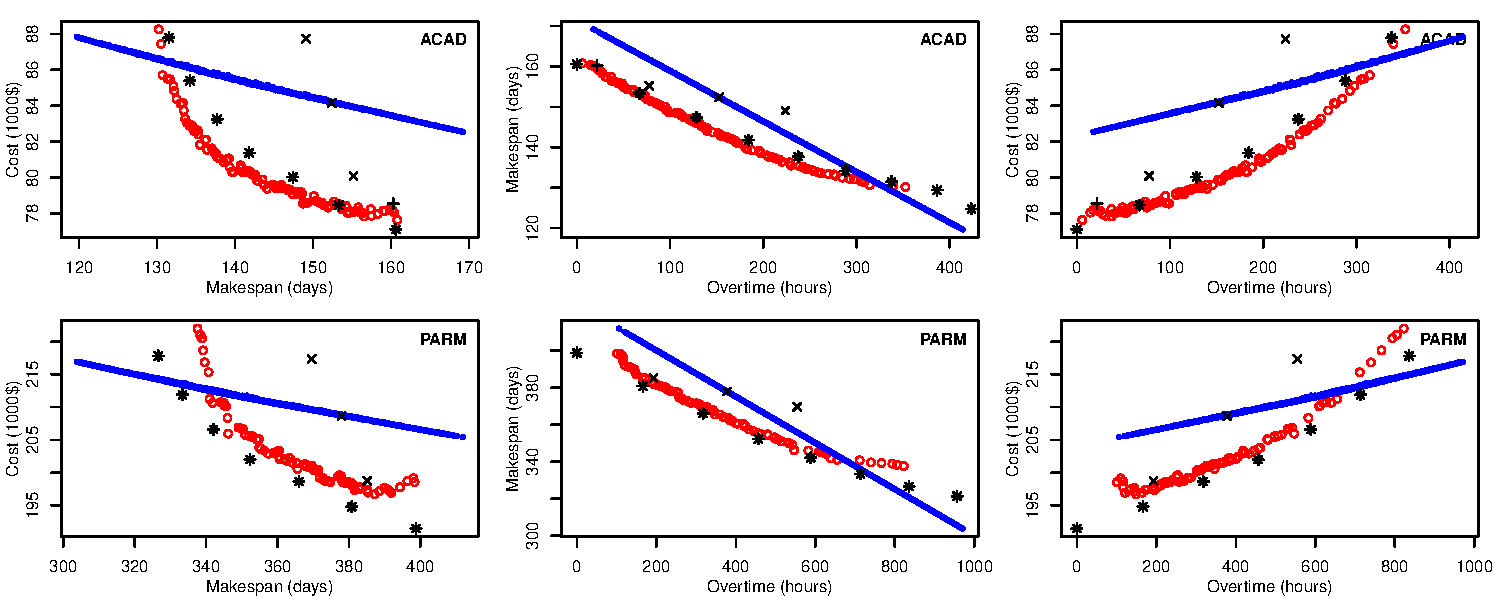
\includegraphics[scale=0.65]{2dplots.pdf}
\caption{2D projections for combinations of the number of overtime hours, makespan, and cost objectives for the smaller (ACAD) and largest (PARM) instances. The linear relations resulting from NSGA$_{NE}$ and the convex shape of NSGA-II can be observed, as well as the few solutions provided by each OMS.}
=======

\textbf{Lessons Learned:} Insights for the decision maker are better appreciated in graphical format. Figure II presents 2D projections of pair-wise combinations for the three objectives comprising our formulation for the OPP. Each chart presents the best Pareto front over 50 optimization cycles under NSGAII (circles), the best Pareto front over 50 cycles under NSGA$_{NE}$ (line), and Pareto fronts for CPM (+), MAR (x), and SH (*). Results are shown for the smallest and the largest instances in our sample (respectively, ACAD and PARM).
%simbolos
A first result that can be observed from these charts is the linear shape of the Pareto front calculated for NSGA$_{NE}$. This front is comprised of a set of points distributed along the main diagonal of the hypercube representing the objective space for the OPP. The shape of the Pareto front implies that there exist linear relationships between the number of overtime hours invested on the project, project makespan and cost if the dynamics in error generation rates is not taken into account. These linear relationships are incompatible with previous findings in Software Engineering research, which postulate an exponential relationship between cost (effort) and duration for non-trivial software projects \cite{Boehm:1981}. They may also make the optimization process easier for the genetic algorithm, resulting in a larger pool of non-dominated solutions and probing parts of the objective space which could not be explored by the more complex search accounting for error dynamics.

\begin{figure*}
\centering
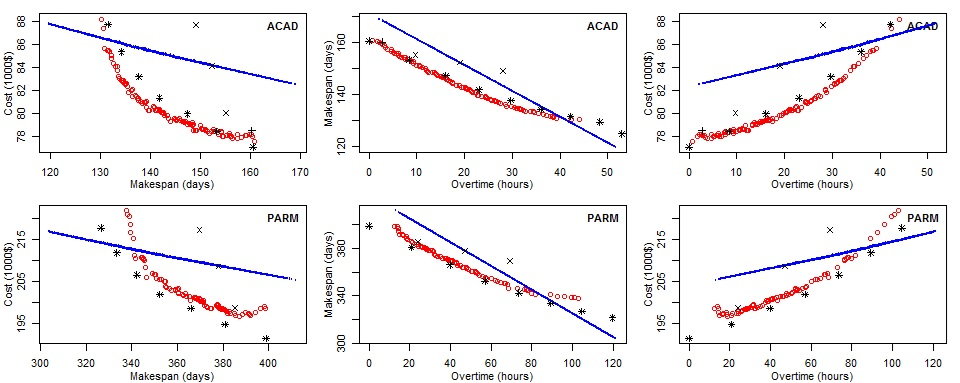
\includegraphics[width=18cm]{lessonslearned.jpg}
\caption{2D projections for combinations of the number of overtime hours, makespan, and cost objectives for the smaller (acad) and largest (parm) instances. the linear relations resulting from NSGA$_{NE}$ and the convex shape of nsga-ii can be observed in the charts, as well as the few solutions provided by each oms.}
>>>>>>> bebbc47c358f93b9cd6e01015a466bf90b44bbfe
\end{figure*}

Other interesting aspect is the convex form of the Pareto fronts resulting from our formulation for the OPP. These fronts also fill the main diagonal of the hypercube representing the objective space, but instead of lines we observe curved distributions of points. These curves can be cut into regions presenting fast decrease/increase in objective values and regions on which changes in objective values are slower. For instance, consider the curves for the PARM instance in the lower part of Figure II. The cost of shrinking makespan below 350 days increases exponentially. To reduce makespan from 350 to 337 days, we have to accept an increase of about 8\% in project cost. On the other hand, reducing makespan from 360 to 350 days requires increasing the cost by only 1.2\%. On regard of overtime hours, the first reduction in makespan requires adding 38 overtime hours to the project, while the second reduction requires adding only 12 hours. 

<<<<<<< HEAD
Knee-points connecting different regions of the Pareto front (such as the one described above) can be explored by decision-makers as overtime allocation alternatives on which large changes in one objective can be garnered by accepting small compromises on other objectives. This allows decision-makers to answer questions such as "what must I do to reduce makespan?", "how much does it cost to reduce makespan by X days?" or "which activities provide the best leverage for a certain amount of overtime?".
=======
Knee-points connecting different regions of the Pareto front (such as the one described above) can be explored by decision-makers' as overtime allocation alternatives on which large changes in one objective can be garnered by accepting small compromises on other objectives. This allows decision-makers to answer questions such as \textit{"what must I do to reduce makespan?", "how much it costs to reduce makespan by X days?" or "which activities provide the best leverage for a certain amount of overtime?"}.

One might question whether we need heuristic search to provide answers to these questions, that is, can't we find these answers relying solely on simulation? We argue that this is not possible because we are interested in relationships between different results from the simulation. If we were interested in relations between parameters and results, we could sample the selected parameters and calculate the distribution of the results under interest. But to calculate the joint distribution of two or more results we would have to sample all parameters, which is equivalent to a complete search (all combinations of possible values are assigned to parameters) or random search (a limited number of combinations are randomly picked and assigned to parameters). Complete search is unfeasible for interesting problems because the size of the solution space is $9^m$, m being the number of activities in the schedule. On the other hand, results from random search are clearly outperformed by our proposed approach, as shown in RQ1. Therefore, heuristic search complements simulation by finding the points in the solution space that represent (close to) optimal combinations of simulation results (in the objective space).
>>>>>>> bebbc47c358f93b9cd6e01015a466bf90b44bbfe

One might question whether we need heuristic search to provide answers to these questions, that is, can't we find these answers relying solely on simulation? We argue that this is not possible because we are interested in relationships between different results from the simulation. If we were interested in relations between parameters and results, we could sample the selected parameters and calculate the distribution of the results under interest. But to calculate the joint distribution of two or more results we would have to sample all parameters, which is equivalent to a complete search (all combinations of possible values are assigned to parameters) or random search (a limited number of combinations are randomly picked and assigned to parameters). Complete search is unfeasible for interesting problems because the size of the solution space is $9^m$, $m$ being the number of activities in the schedule. On the other hand, results from random search are clearly outperformed by our proposed approach, as shown in RQ1. Therefore, heuristic search complements simulation by finding the points in the solution space that represent (close to) optimal combinations of simulation results (in the objective space).

Regarding the last question presented above, we observe strong concentration of overtime allocation in coding and testing activities in Pareto fronts calculated for NSGAII. This concentration is consistent with error dynamics: an increase in the number of errors produced in requirement analysis or design will snowball through the subsequent activities, increasing the cost of testing later in the schedule. Here the extensible nature of simulation provide us an interesting opportunity: one can break error propagation dynamics by using formal reviews or inspections to identify and correct errors earlier than while testing the software. The proposed simulation mechanism allows developing a scenario to represent the effects of such activities \cite{Madachy:1996} and combine them with error dynamics. The concentration of overtime in later activities is also consistent with the quality of the Pareto front built for the SH OMS. As can observed in Figure II, the Pareto front for SH has few points, but it is close to the front built for NSGAII, sometimes even showing better fitness (i.e., PARM instance). Therefore, SH can be used as a starting point for the decision-maker and can be enriched by merging its results with those calculated using our approach.

Finally, despite of having different shapes in the objective space, NSGA and NSGA$_{NE}$ present extremely high inverse correlation between the number of overtime hours and project makespan (close to -1.0 Spearman rank-order index). NSGA$_{NE}$ also presents extremely high correlation between all pairs of objectives. This leads to actionable results in the sense that algorithms might not be required to pursue optimal values for all three objectives, but only two of them: minimum makespan is observed in solutions having maximum overtime. In practical terms, discarding one objective reduces the cost of optimization, allowing for more generations to be considered and a more diverse number of solutions to be found on Pareto fronts produced by NSGAII.

\noindent
\textbf{Validity Threats:} The design of the experimental study has taken into account potential sources of validity threats, including dealing with the randomness inherent to heuristic algorithms (all heuristic algorithms were executed 50 times before comparisons were made) and selecting proper statistical inference tests and effect-sizes for analysis (non-parametric tests and effect-sizes were used, since the data to be analyzed would not present Gaussian distribution). However, the study is not completely immune to validity threats.

One important validity threat is related to external validity, that is, our ability to generalize observed results to other contexts. The study presented above is based on a schedule generation strategy and a set of parameters that were used in the overtime scenario. These parameters may not represent the reality of all software development companies and should be collected on a company basis to allow for more precise results. Companies hiring more experienced developers, using formal inspections or other V\&V strategies may be able to introduce fewer errors or identify and correct them earlier in the life-cycle, becoming more resilient to the effects of overtime.

Simulation also adds validity threats of its own, including the use of a non-infinitesimal simulation step for continuous simulation (if a larger simulation step is used to fasten objective values calculation during the optimization) or rounding problems (if a smaller step is adopted). The need to find a balance between the computational effort required to produce simulation results and their precision may also be considered a validity threat. On its turn, optimization may also require more fitness evaluations as stop criteria, thus leading to a reevaluation of other parameters, such as population size.

\section{Related Works}

Continuous-time simulation has been extensively used to model software projects, most notably by the seminal work of Abdel-Hamid and Madnick \cite{Abdel-Hamid:1991}, who presented a System Dynamics model of a software project following a waterfall life-cycle and comprising more than 270 equations. Later, this model was extended by Tvedt \cite{Tvedt:1996}, who added equations to describe a concurrent and incremental life-cycle model. Lin et al. added requirement volatility, milestones, and the possibility to discard certain activities comprising the schedule due to lack of resources \cite{Lin:1997}. Madachy \cite{Madachy:1996} used System Dynamics to describe the behavior of inspections on software projects. Recently, Cao et al. \cite{Cao:2010} have used simulation models to evaluate the effects of practices suggested by agile processes.

Optimization has also been combined with simulation for project planning purposes. Harman et al. \cite{harman:2009} presents a general framework for project planning optimization that uses a simulator to calculate fitness functions according to a project plan and a set of constraints for staff allocation. Antoniol et al. \cite{Antoniol:2004} combine a genetic algorithm with a queuing simulator to optimize staff allocation and work package ordering on software projects. The simulator calculates project makespan taking into consideration uncertainties about the effort required for each activity, rework and abandonment of work packages. Recently, Rodriguez et al. \cite{Rodriguez:2011} used System Dynamics models in conjunction with NSGAII to find ideal team size and schedule estimations for a software project.

\section{Conclusion and Future Work}

In this paper we introduced a formulation for the overtime-planning problem that uses a multi-objective search-based approach and takes into account both positive and negative aspects of overtime. Continuous simulation is used to mimic the behavior of a software project under different conditions of overtime allocation. We compared the proposed approach with practices from the industry and with a similar formulation without the negative effects on quality. 

We observed that our approach performs significantly better (high effect-size) than the margarine and critical-path overtime-allocation strategies. However, the practice that suggests allocating overtime in the second half of the project's schedule is competitive with our approach and may lead to good overtime allocations, specially in large projects. This behavior confirms the "gut-feeling" of practitioners who tend to allocate overtime in the last activities to compensate for earlier delays. Therefore, by combining search-based optimization and software project simulation we can help researchers to design experimental studies to investigate, evaluate, and provide scientific support for practices and assumptions used in the industry, converting intuition into evidence-based knowledge. 

For future work, we consider creating new simulation scenarios to model other aspects of software projects, such as exhaustion due excessive overtime, learning curve, inspections, among others. We also intend to integrate the approach with project management tools, allowing further experimental analysis, particularly to engage humans with the tool and observe their reaction to the overtime allocations it suggests. We also believe that creating means to help visualizing the differences among the overtime allocations proposed by NSGAII is an important aspect towards adopting our approach in practice.

%\section{Acknowledgment}

\bibliography{Article}
\bibliographystyle{IEEEtran}

\end{document}
